\documentclass[a4paper,12pt]{article}

\usepackage[utf8]{inputenc}
\usepackage[T1]{fontenc}
\usepackage[french]{babel}
\usepackage[sfdefault]{roboto}
\usepackage[protrusion=true,expansion=true]{microtype} 
\usepackage{csquotes}

\usepackage[top=2.5cm, bottom=2.5cm, left=2.5cm, right=2.5cm]{geometry}
\usepackage{fancyhdr}
\usepackage{lastpage}
\usepackage{float}
\usepackage{parskip}

\usepackage{graphicx}
\usepackage{xcolor}
\usepackage{tikz}

\definecolor{primaryColor}{RGB}{0, 50, 100}
\definecolor{accentColor}{RGB}{180, 20, 40}
\definecolor{codeBack}{RGB}{245, 245, 245} 
\definecolor{codeGreen}{RGB}{0, 150, 0}
\definecolor{codeGray}{RGB}{100, 100, 100}
\definecolor{codePurple}{RGB}{120, 0, 120}


\usepackage{booktabs} 
\usepackage{array}
\usepackage{tabularx}
\usepackage{enumitem} 

\usepackage{amsmath}
\usepackage[linesnumbered,ruled,vlined]{algorithm2e}
\usepackage{listings}

\usepackage{hyperref}
\hypersetup{
    colorlinks=true,
    linkcolor=primaryColor,
    filecolor=magenta,      
    urlcolor=accentColor,
    citecolor=accentColor,
    pdftitle={Rapport de Projet : Modernisation du Réseau Alumnis},
    pdfauthor={Benoît, Joris, Robin, Théo}
}


\usepackage{titlesec}
\titleformat{\section}
  {\color{primaryColor}\normalfont\Large\bfseries}
  {\thesection}{1em}{}[\titlerule]
  
\titleformat{\subsection}
  {\color{primaryColor}\normalfont\large\bfseries}
  {\thesubsection}{1em}{}

\titleformat{\subsubsection}
  {\color{primaryColor}\normalfont\normalsize\bfseries}
  {\thesubsubsection}{1em}{}

\pagestyle{fancy}
\fancyhf{}
\fancyhead[L]{\small \textsc{Projet Informatique}}
\fancyhead[R]{\small \textbf{Modernisation Réseau Alumnis}}
\fancyfoot[L]{\small ENSICAEN}
\fancyfoot[C]{\thepage\ / \pageref{LastPage}}
\fancyfoot[R]{\small 2025-2026}
\renewcommand{\headrulewidth}{0.4pt}
\renewcommand{\footrulewidth}{0.4pt}


\begin{document}

\begin{titlepage}
    \thispagestyle{empty}
    \newgeometry{top=2cm, bottom=2cm, left=2cm, right=2cm}
    
    \begin{minipage}{0.4\textwidth}
        
\includegraphics[height=3.5cm]{images/ENSICAEN - logotype couleur.png} 
        
    \end{minipage}
    \hfill
    \begin{minipage}{0.55\textwidth}
        \raggedleft
        \color{primaryColor}
        \textbf{\large ENSICAEN}\\
        \textit{Projet Informatique}\\
        \textit{Spécialité Informatique}
    \end{minipage}

    \vspace{3cm}

    \begin{center}
        \rule{\linewidth}{0.5mm} \\[0.6cm]
        {\fontsize{24}{30}\selectfont \bfseries \textsc{Modernisation du\\ Réseau Alumnis}} \\[0.4cm]
        \rule{\linewidth}{0.5mm} \\[1.5cm]
        
        {\Large \textbf{Rapport de Projet}}
    \end{center}

    \vspace{1cm}

    \begin{center}
        \large
        \textbf{Clients :} Association Alumnis \\[0.3cm]
        \textbf{Tuteur École :} Hélène le Bouteille
    \end{center}

    \vfill

    \begin{center}
        \large \textbf{Équipe de Développement} \\[0.3cm]
        \begin{tabular}{c c}
             Cheramy Benoit & Moczygeba Joris \\
             Molle Robin & Gicquel Théo
        \end{tabular}
    \end{center}
    
    \vspace{1cm}
    \centering
    
    \restoregeometry
\end{titlepage}

\newpage
\thispagestyle{empty}
{
    \hypersetup{linkcolor=black}
    \tableofcontents
}
\newpage

\setcounter{page}{1}

\section{Présentation du projet : De l'annuaire à la plateforme communautaire}

\subsection{La mission initiale : Faciliter le contact}
À l'origine, le projet consistait à répondre à un besoin technique précis : la création d'un annuaire électronique permettant une mise en relation directe et fluide entre les étudiants actuels et les Alumnis. L'objectif premier était de remplacer les outils existants par une solution numérique, en transformant un fichier statique en un outil de recherche dynamique pour favoriser le tutorat et le conseil professionnel.

\subsection{Évolution de la vision : Promouvoir l'excellence du réseau}
Au cours des premiers échanges, le besoin du client a rapidement évolué. Plus qu'un simple outil de contact interne, l'ambition est devenue celle de créer une véritable plateforme de promotion.

\begin{itemize}[label=\textbullet, itemsep=5pt]
    \item \textbf{Rayonnement interne :} Sensibiliser les étudiants à la force et à la diversité du réseau actuel.
    \item \textbf{Visibilité externe :} Valoriser le parcours des anciens de l'ENSICAEN auprès des partenaires extérieurs et des futurs candidats.
\end{itemize}

Cette volonté s'est traduite par le passage d'une application utilitaire à un support d'information complet, accessible à tout utilisateur souhaitant découvrir le dynamisme de la communauté.

\subsection{État des lieux}
Avant de débuter le développement, une phase d'analyse a été menée :

\begin{itemize}[label=\textbullet, itemsep=5pt]
    \item \textbf{Constat interne :} Le site existant des Alumnis a été identifié comme "sous-utilisé" et esthétiquement dépassé. La centralisation des données était inefficace pour les besoins actuels des étudiants. La multiplication d’accès aux différentes bases de données rend complexe toute recherche pour un étudiant entrant dans l’école.
    \item \textbf{Benchmark externe :} Nous avons étudié les solutions de structures aux moyens similaires (écoles d'ingénieurs) mais aussi de références d'excellence comme l'EM Normandie ou Sciences Po Paris. Elles avaient toutes en commun la centralisation de plusieurs outils sur leur page internet (offre, actualité des Alumnis,...).
    \item \textbf{Fait aggravant de conformité (RGPD) :} Lors de l'audit, nous avons mis en évidence une faille critique liée à l'utilisation des données personnelles et à la possibilité de les exporter. Le calendrier des stages de 2\textsuperscript{e} année, exposait les données d'étudiants transmises (noms, entreprises, contacts) et affichées sans leur consentement explicite.    
\end{itemize}

Face à l'obsolescence des outils actuel, nous avons obtenu l'accord du client pour \textbf{partir d'une page vierge} afin de garantir une architecture propre, évolutive et conforme aux attentes des utilisateurs.

\subsection{Des fonctionnalités au service de l'engagement}
En concertation avec le client, plusieurs piliers fonctionnels ont été ajoutés pour garantir que la plateforme devienne le cœur battant du réseau :

\begin{itemize}[label=\textbullet, itemsep=5pt]
    \item \textbf{L'annuaire intelligent et qualifié :} Pivot central du projet, cet annuaire ne se contente pas de recenser des noms. À la demande du client, il intègre des données stratégiques pour l'étudiant : la filière suivie à l'école, l’entreprise actuelle de la personne mais aussi le détail des stages de 2A et 3A réalisés. Ces informations permettent un ciblage précis pour ceux qui cherchent des conseils sur une spécialité ou un retour d'expérience sur une entreprise spécifique.
    \item \textbf{La cartographie des entreprises :} À la suite de nos échanges, nous avons intégré une dimension géographique au projet. L'outil propose une carte des entreprises représentées au sein du réseau. Cette interface permet de visualiser en un coup d'œil l'influence des Ensicannais sur le territoire et d'identifier les bassins d'emploi où la communauté est la plus présente.
    \item \textbf{Le volet "Carrière" :} À notre initiative, nous avons intégré un module de dépôt d'offres de stages et d'emplois. Cette fonctionnalité crée un cercle vertueux d'entraide, facilitant directement l'employabilité des Ensicannais et renforçant l'utilité concrète du réseau au quotidien.
    \item \textbf{Gestion de l'actualité et des événements :} Un espace dédié permet à l'association d'administrer du contenu de manière autonome. Cet outil mettra en lumière l'engagement des anciens étudiants et diffusera les événements clés, garantissant un réseau vivant et ouvert à toute proposition d’évènement.
\end{itemize}

\subsection{Un cadre technique responsable : Contrainte RGPD}
Le développement de cette plateforme s'est fait sous une contrainte majeure et structurante : le respect du RGPD (Règlement Général sur la Protection des Données). Le projet intègre nativement la gestion du consentement des Alumnis pour la diffusion de leurs informations et assure un cloisonnement strict des données personnelles. L'enjeu technique a été de concilier la visibilité nécessaire à la promotion du réseau avec la protection absolue de la vie privée des membres, notamment lors de la phase de ciblage des contacts par les étudiants.

\newpage

\section{Objectifs du Projet}

\subsection{La phase de développement : Most Valuable Product}
La première étape de notre mission s’est concentrée sur la mise en place d'un socle technique robuste et fonctionnel, répondant aux besoins les plus immédiats des utilisateurs. L'objectif prioritaire a été la structuration d'une base de données capable de centraliser les informations des anciens élèves tout en garantissant une sécurisation et une conformité totale avec les réglementations européennes sur la protection des données personnelles (RGPD). Cela a permis de déployer un annuaire électronique performant, conçu pour offrir aux étudiants des outils de recherche multicritères. Grâce à ce système, les utilisateurs peuvent cibler des contacts pertinents en fonction de secteurs d'activité, d'entreprises ou de spécialités précises, tout en préservant la confidentialité des membres grâce à un affichage partiel des informations et au masquage des coordonnées privées.

Parallèlement à cet outil de recherche, cette phase de lancement a intégré un module de mise en relation directe. Ce système a pour but de faciliter l'organisation des interventions historiques de l'association, telles que les "Rencontres du samedi", tout en ouvrant une voie pour solliciter des conseils personnalisés en matière de recrutement.

\subsection{La vision à long terme : la plateforme communautaire intégrale}
Au-delà des fonctionnalités de base, le projet vise à transformer cet outil en une plateforme communautaire complète, servant de vitrine d'excellence pour l'ENSICAEN. L'un des objectifs finaux essentiels est de mettre en avant l'engagement des Alumnis afin de valoriser le dynamisme et le rayonnement de l'école, tant auprès des étudiants que des partenaires extérieurs. Pour garantir la pérennité et l'animation de ce réseau, nous avons conçu une interface d'administration intuitive spécifiquement dédiée, permettant à la secrétaire de l'association de mettre à jour le contenu. Cet outil lui permet de gérer de manière autonome un espace consacré aux actualités et aux événements, assurant ainsi une communication fluide et régulière qui fait vivre la communauté.

Enfin, la dimension professionnelle de la plateforme trouve son aboutissement dans l'intégration d'un module dédié à l'employabilité. Ce volet permet aux anciens de déposer directement des offres de stages et d'emplois au sein d'un espace exclusif réservé aux étudiants et diplômés de l'école. En favorisant ce circuit court du recrutement, le projet ne se contente plus d'être un simple annuaire, mais devient un levier stratégique pour l'insertion professionnelle des Ensicannais, renforçant concrètement la solidarité intergénérationnelle du réseau.

\newpage

\section{Méthodologie et Organisation du Travail}

\subsection{Un pilotage adaptatif : la méthodologie Agile}
Pour mener à bien ce projet, nous avons fait le choix d'une méthodologie Agile. Ce cadre de travail s'est révélé indispensable pour répondre à la nature évolutive des besoins de l'association Alumnis. Contrairement à une approche séquentielle rigide, l'agilité nous a offert la flexibilité nécessaire pour réorienter nos efforts lorsque le périmètre fonctionnel a évolué.

Ce changement d'orientation, marquant le passage d'un simple annuaire à une plateforme complète de promotion du réseau, a été intégré de manière fluide au cycle de production. La réussite de cette transition repose sur l'adoption d'itérations courtes, d'une durée d'une à deux semaines par rendu, et sur un dialogue permanent avec le client.

La mise en place de cette organisation a été grandement facilitée par la journée de formation \og Gestion de projet Agile \fg{} dispensée à l'école. Cet atelier pratique nous a fourni les outils méthodologiques nécessaires pour découper efficacement le projet en sous-tâches réalisables (\textit{User Stories}) et pour cartographier précisément les différents acteurs (étudiants, Alumnis, administration, DSI) avec lesquels nous allions interagir tout au long du développement.

\subsection{Structure de l'équipe et responsabilités}
L'efficacité du groupe a reposé sur une répartition claire des compétences, permettant à chaque membre de se concentrer sur des domaines d'expertise tout en collaborant sur le développement global :

\begin{itemize}[label=\textbullet, itemsep=5pt]
    \item \textbf{Benoît}, en tant que chef d'équipe, a assuré la coordination générale du projet et le respect des délais. Il a également pris en charge la dimension design (UI/UX) pour garantir une interface moderne, tout en participant activement aux phases de développement.
    \item \textbf{Joris}, occupant le rôle de développeur Full Stack, a été le pivot technique entre la structure des données et l'interface utilisateur, intervenant sur l'ensemble de la chaîne de programmation pour assurer la cohérence du système.
    \item \textbf{Robin} a combiné ses missions de développement avec la gestion du dépôt de code (Git). Sa responsabilité a consisté à maintenir l'intégrité des versions du projet, à organiser les fusions de code et à garantir un environnement de travail stable pour l'ensemble du groupe.
    \item \textbf{Théo} s'est concentré sur les aspects critiques liés au développement et à la sécurité. Son rôle a été particulièrement déterminant dans la mise en œuvre des protocoles de protection des données, assurant que chaque fonctionnalité développée respecte les standards de sécurité de l'ANSSI et les contraintes réglementaires du RGPD.
\end{itemize}

\subsection{Gestion du flux de travail : le système Kanban}
Pour organiser notre production de manière visuelle et transparente, nous avons mis en place un tableau Kanban, intégré nativement dans le GitLab de l’Ensicaen. Cet outil de gestion de flux nous a permis de segmenter le travail en plusieurs étapes distinctes, garantissant ainsi une progression constante et une identification rapide des éventuels points de blocage.

\begin{figure}[H]
    \centering
    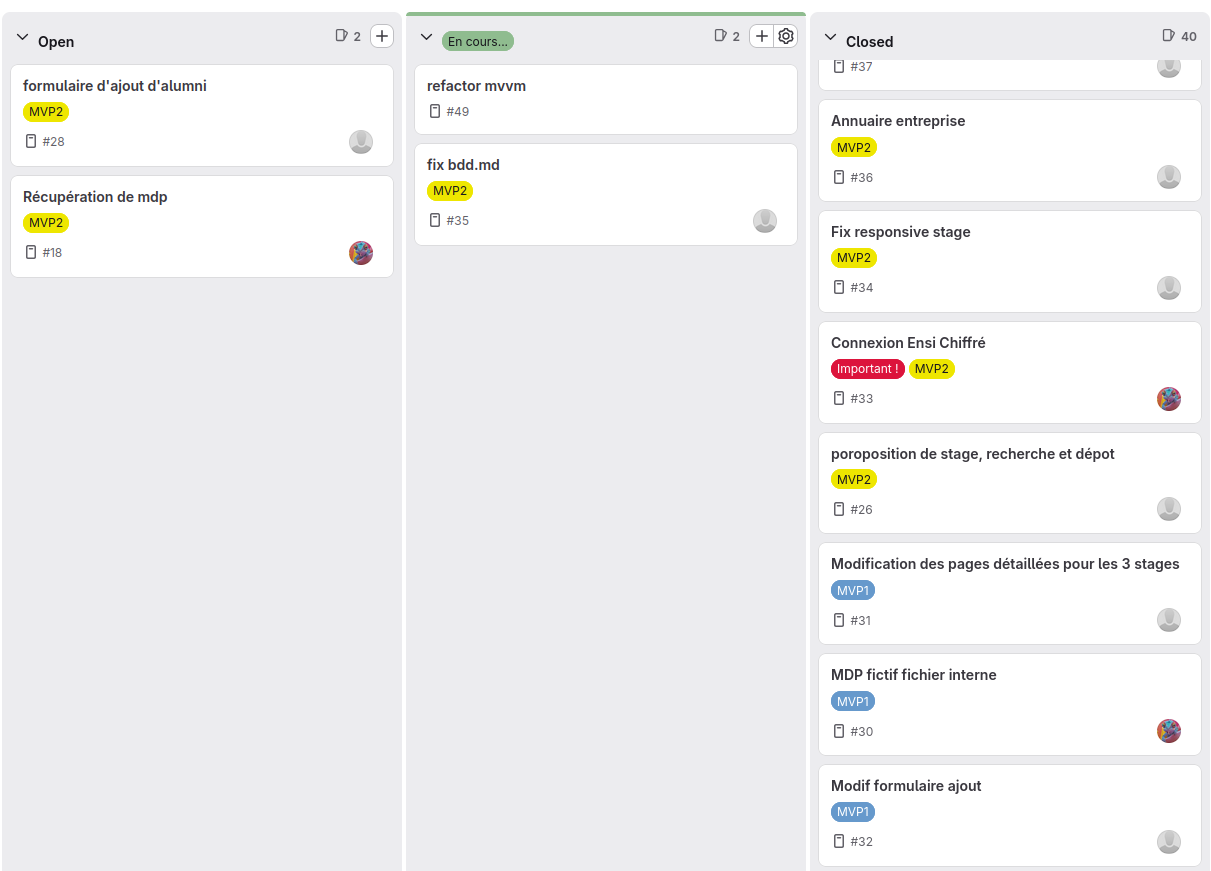
\includegraphics[width=0.9\textwidth]{images/kanban.png} 
    \caption{Aperçu du tableau Kanban utilisé pour la gestion du projet.}
    \label{fig:kanban}
\end{figure}

Le cycle de vie de nos tâches s'est articulé autour de trois colonnes majeures. L’identifications des besoins avec le client, tels que la promotion de l’école, la mises en correspondance des Alumnis avec les élèves ou encore l'annuaire. Ces tâches étaient ensuite découpées en plusieurs sous-tâches avant de les traiter individuellement dans la partie “En cours”, où elles faisaient l'objet d'un développement intensif (notamment sur les modules de sécurité, d'authentification et les moteurs de recherche). Enfin, son passage définitif dans la colonne \textit{Terminé} marquait la validation officielle de la fonctionnalité et son intégration au produit final.

\subsection{Choix Technologiques et Architecture}
Pour garantir la maintenabilité, l'évolutivité et la performance de la plateforme, nous avons structuré notre développement autour de choix technologiques et de patrons de conception (\textit{Design Patterns}) robustes :

\begin{itemize}[label={\color{accentColor}\textbullet}, itemsep=5pt]
    \item \textbf{Technologie Multiplateforme (Dart \& Flutter) :} Afin de maximiser la portée du projet tout en optimisant le temps de développement, nous avons opté pour le langage \textbf{Dart}. Son atout majeur est de permettre la création d'applications Web, Android et iOS à partir d'une \textbf{seule et même base de code}. Ce choix stratégique garantit à l'association une couverture maximale avec un coût de maintenance minimal. De plus, le typage fort de Dart sécurise la logique métier, tandis que ses outils de développement (comme le \textit{Hot Reload}) se sont parfaitement intégrés à notre démarche Agile en accélérant les itérations sur le design de l'interface (UI/UX).

    \item \textbf{Architecture MVVM (Model-View-ViewModel) :} En adéquation avec notre choix de langage, nous avons séparé la logique métier (Modèle), l'interface utilisateur (Vue) et la logique de présentation (ViewModel). Ce choix permet de découpler totalement le rendu visuel de la gestion des données, facilitant ainsi le travail simultané de l'équipe sur le front-end et le back-end sans créer de conflits, tout en rendant le code plus facilement testable.

    \item \textbf{Patrons Stratégie et Adaptateur (Authentification) :} La gestion de la connexion s'appuie sur le patron \textit{Stratégie}, permettant de basculer dynamiquement entre plusieurs méthodes d'authentification (comptes locaux vs. comptes Microsoft institutionnels) sans modifier le cœur de l'application. Cette flexibilité laisse également la possibilité d'ajouter facilement d'autres méthodes de connexion futures souhaitées par le client comme LinkedIn. Pour intégrer l'API Microsoft Graph, nous avons couplé cette stratégie à un patron \textit{Adaptateur}, chargé de traduire les données brutes renvoyées par Microsoft (jetons OAuth) dans le format standard attendu par notre base d'utilisateurs interne.
\end{itemize}

\newpage

\section{Bilan du Projet : Réalisations et Gestion des Aléas}

\subsection{Bilan Technique et Fonctionnel}
Au terme du cycle de développement, l'équipe a livré une solution répondant aux exigences majeures du cahier des charges. Le travail s'est articulé autour de quatre axes techniques :

\begin{itemize}[label=\textbullet, itemsep=5pt]
    \item \textbf{Le moteur de recherche} Alumnis couplé à différents filtres permettant un ciblage précis.
    \item \textbf{La protection des données} a été intégrée dès la conception. Le système assure la gestion du consentement et applique un masquage rigoureux des données sensibles tant que la mise en relation n'a pas été validée. L’utilisateur doit être authentifié pour avoir accès à différents types de données afin de respecter le cadre strict du RGPD.
    \item \textbf{Le module "Carrière"} permettant le dépôt et la consultation d'offres de stages et d'emplois, afin de transformer la plateforme en un véritable hub d’embauche pour les Ensicannais.
    \item \textbf{Une interface d'administration simplifiée} a été mise à la disposition de l'association permettant au secrétariat de gérer les actualités et les événements en totale autonomie, sans intervention technique.
\end{itemize}

\subsection{Gestion des obstacles et résilience technique}
Le projet a été confronté à des défis critiques qui ont nécessité une réorientation technique majeure.

\subsubsection{Pivot d'infrastructure : Le défi de la souveraineté des données}
L'obstacle le plus significatif a été l'impossibilité d'accéder aux bases de données initialement promises, suite à des restrictions pour des raisons de sécurité.

Face à cette impasse qui aurait pu paralyser le projet, le groupe a fait preuve d'une autonomie totale :
\begin{itemize}[label=\textbullet, itemsep=5pt]
    \item \textbf{Conception d'une infrastructure propre :} Nous avons développé et déployé une base de données MySQL indépendante pour pallier l'absence de sources externes.
    \item \textbf{Administration serveur :} L'hébergement a été configuré sur un serveur dédié, administré via phpMyAdmin, pour centraliser l'information de manière sécurisée.
    \item \textbf{Simulation de données :} Afin de valider la viabilité de notre code et de démontrer les fonctionnalités du site, nous avons généré l'intégralité d'un schéma relationnel (tables) et créé des jeux de données fictives. Ce travail a permis de prouver que la plateforme est prête à accueillir les données réelles dès que les protocoles d'accès seront rétablis.
\end{itemize}

\subsubsection{Sécurité et Authentification Microsoft}
L'une des ambitions techniques du projet était d'intégrer un système de double authentification, calqué sur le fonctionnement de la plateforme FOAD de l’ENSICAEN. Ce volet visait à permettre une connexion fluide via les comptes Microsoft institutionnels des utilisateurs.

Cependant, cette intégration a représenté un défi d'une complexité majeure, marqué par des contraintes d'infrastructure insurmontables :
\begin{itemize}[label=\textbullet, itemsep=5pt]
    \item \textbf{Restrictions de la DSI :} La configuration des flux OAuth 2.0 via l'API Microsoft Graph nécessite la création d'un emplacement d'application (App Registration) sous l'autorité de la DSI de l'école. Pour des raisons de sécurité — notamment le cloisonnement entre les projets étudiants et le réseau professionnel de l'établissement — cet accès n'a pas pu nous être accordé.
    \item \textbf{Échec des solutions de contournement :} Nous avons tenté de contourner ce blocage en utilisant des comptes personnels. Toutefois, ces derniers étant techniquement liés à l'annuaire de l'école (tenant Microsoft), ils héritaient des mêmes restrictions de sécurité, empêchant ainsi tout déploiement en dehors du cadre administré par la DSI.
\end{itemize}

Malgré ces obstacles, un travail de recherche approfondi a été mené sur la sécurisation des flux OAuth et la gestion granulaire des permissions. L'enjeu était de concevoir un système garantissant une expérience utilisateur simplifiée tout en maintenant un haut niveau de sécurité pour les accès administratifs.

En raison de l'impossibilité d'obtenir les autorisations nécessaires, la couche d'authentification Microsoft n'a pas pu être testée en environnement réel. Elle demeure toutefois intégrée au prototype sous forme de "Preuve de Concept" (PoC), démontrant la viabilité théorique de la solution pour une éventuelle implémentation future si les accès venaient à être ouverts.

\subsection{Facteurs de succès}

\subsubsection{Cohésion et synergie du groupe}
L'un des piliers fondamentaux de la réussite de ce projet a été l'excellente entente au sein de l'équipe dès le premier jour. Au-delà d'une simple collaboration professionnelle, le groupe est constitué d'amis, ce qui a naturellement instauré un climat de confiance, d'honnêteté et de transparence totale entre nous. Cette proximité a permis de supprimer les barrières de communication et s'est traduite par une efficacité opérationnelle réelle :
\begin{itemize}[label=\textbullet, itemsep=5pt]
    \item \textbf{Communication sans filtre et Résolution proactive :} Grâce à notre complicité, nous avons pu identifier les obstacles techniques et organisationnels très tôt. L'honnêteté mutuelle nous a permis de nous dire les choses directement, facilitant ainsi une communication interne fluide.
    \item \textbf{Agilité décisionnelle :} Chaque problème rencontré a fait l'objet d'une analyse collective sincère, permettant de faire émerger rapidement des solutions concrètes, partagées et validées par tous sans ambiguïté.
\end{itemize}

\subsubsection{Communication client}
Nous avons maintenu un dialogue constant et transparent avec notre client. Cette démarche a été cruciale pour :
\begin{itemize}[label=\textbullet, itemsep=5pt]
    \item \textbf{Gérer les attentes :} Expliquer de manière pédagogique les limitations techniques imposées par les contraintes de sécurité de la DSI.
    \item \textbf{Réorientation stratégique :} Obtenir l'aval pour réorienter les objectifs du projet vers une infrastructure autonome sans perdre la valeur ajoutée finale pour l'utilisateur.
\end{itemize}

\subsubsection{Adaptabilité et résilience technique}
Le groupe ne s'est pas laissé paralyser par l'absence des ressources initialement prévues. Notre capacité à pivoter d'un projet de "traitement de données existantes" vers un projet de "création complète d'architecture" (Base de données, API, Serveur) est le point positif majeur de notre fonctionnement. Cette transition a démontré notre autonomie et notre capacité à livrer un système fonctionnel malgré un environnement instable.

\subsubsection{Excellence du rendu : Sécurité et Design}
Malgré les défis structurels, nous avons mis un point d'honneur à livrer une plateforme aboutie qui ne fait aucun compromis sur la qualité :
\begin{itemize}[label=\textbullet, itemsep=5pt]
    \item \textbf{Interface utilisateur (UI/UX) soignée :} Nous avons développé une plateforme au design propre, moderne et intuitif. L'utilisation de thèmes cohérents (ENSICAEN Alumni) assure une expérience utilisateur professionnelle.
\item \textbf{Architecture sécurisée (\textit{Security by Design}) :} La cybersécurité a constitué un enjeu central de notre développement afin de répondre aux exigences strictes du RGPD. Outre l'intégration de Microsoft Auth, l'authentification locale par mot de passe a été sécurisée via une fonction de hachage robuste avec ajout de sel (\textit{salt}), en parfaite conformité avec les recommandations de l'ANSSI. De plus, la gestion des sessions s'appuie sur des jetons cryptographiques (tokens JWT). Ce mécanisme certifie l'identité de l'utilisateur à chaque requête et empêche toute falsification de ses droits d'accès, démontrant notre engagement absolu dans la protection des données de la communauté.\end{itemize}

\subsection{Analyse des résultats}
Malgré les contraintes extérieures, les objectifs principaux sont atteints :
\begin{itemize}[label=\textbullet, itemsep=5pt]
    \item \textbf{Centralisation :} Les données, autrefois dispersées, sont désormais structurées dans un environnement unique.
    \item \textbf{Modernité :} L'interface offre une expérience utilisateur conforme aux standards actuels, dépassant largement les capacités de l'ancienne solution.
    \item \textbf{Autonomie :} Le client dispose désormais d'un outil "clés en main" pour faire vivre la communauté.
\end{itemize}

\newpage

\section{Perspectives et axes d’améliorations}
Afin de pérenniser et d'enrichir la dynamique de communauté, nous avons identifié plusieurs axes d’évolution stratégiques permettant de projeter la plateforme au-delà de son stade actuel de MVP.

\subsection{Approfondissement de la mise en relation (Mentorat)}
Le document de cadrage soulignait l'importance de tracer les échanges. Nous pourrions aller plus loin en intégrant :
\begin{itemize}[label=\textbullet, itemsep=5pt]
    \item \textbf{Module de Mentorat complet :} Mettre en place un suivi qualitatif et quantitatif des relations de coaching (orientation pour les FISE 2A/3A, recrutement pour les MTS).
    \item \textbf{Évaluation et Feedback :} Intégrer un système de notation ou de témoignages après une rencontre (comme les "Rencontres du samedi") pour mesurer l'impact de l'accompagnement et encourager de nouveaux Alumnis à devenir mentors.
\end{itemize}

\subsection{Synchronisation et rayonnement professionnel}
\begin{itemize}[label=\textbullet, itemsep=5pt]
    \item \textbf{Intégration avec LinkedIn :} Créer une synchronisation bidirectionnelle avec LinkedIn pour maintenir les profils à jour automatiquement et renforcer la visibilité de la vitrine de l'école, qui compte déjà plus de 6 200 abonnés.
    \item \textbf{Valorisation des projets industriels :} Ajouter une section dédiée aux projets de recherche en Intelligence Économique (IE) ou aux projets de fin d'études. Cela permettrait aux étudiants de promouvoir leur expertise auprès des Alumnis et aux entreprises de repérer des talents sur des sujets concrets.
\end{itemize}

\subsection{Visualisation de la visibilité des informations}
\begin{itemize}[label=\textbullet, itemsep=5pt]
    \item \textbf{Gestion granulaire du RGPD :} Bien que le MVP respecte déjà la protection des données, une version future pourrait offrir aux Alumnis un tableau de bord précis pour gérer la visibilité de leurs coordonnées privées, tout en permettant aux étudiants d'être acteurs de la prise de contact de manière tutorée.
\end{itemize}

\subsection{Internationalisation et ouverture globale}
L'application intègre nativement un système d'internationalisation complet (Français/Anglais), permettant une navigation fluide pour les Alumnis basés à l'étranger. Cette fonctionnalité a été implémentée via un \texttt{LocaleProvider} et un sélecteur de langue dynamique en temps réel. Pour aller plus loin, nous envisageons :
\begin{itemize}[label=\textbullet, itemsep=5pt]
    \item \textbf{Traduction dynamique des données (Backend) :} Actuellement, si l'interface est traduite, les données provenant de la base de données (intitulés de postes, secteurs d'activité, chiffres clés) restent dans leur langue de saisie. L'évolution logique serait d'implémenter un stockage bilingue en base de données pour assurer une cohérence totale de l'expérience utilisateur, quelle que soit la langue choisie.
\end{itemize}

\newpage

\section{Ressources et Outils}
\begin{itemize}[label={\color{accentColor}\textbullet}, itemsep=5pt]
    \item \textbf{Environnement de développement et Hébergement :} 
    \begin{itemize}
        \item Serveur dédié et base de données MySQL autonome.
        \item Administration via phpMyAdmin.
    \end{itemize}
    
    \item \textbf{Technologie et Programmation :} 
    \begin{itemize}
        \item Langage Dart et framework Flutter pour le développement multiplateforme.
    \end{itemize}

    \item \textbf{Gestion de projet :} 
    \begin{itemize}
        \item Méthodologie Agile et itérations courtes.
        \item Tableau Kanban intégré au GitLab de l'ENSICAEN.
        \item Versioning et gestion du code collaboratif via Git.
    \end{itemize}

    \item \textbf{Intelligence Artificielle Générative :}
    \begin{itemize}
        \item \textbf{Gemini :} Assistance à la structuration, à la révision et à la mise en page avancée du rapport en LaTeX et certaines partie de code Dart \& Flutter. Utilisation ponctuelle pour la clarification de concepts d'architecture logicielle (MVVM, Design Patterns) et l'aide au débogage.
    \end{itemize}

    \item \textbf{Recherche et Documentation :}
    \begin{itemize}
        \item Documentation officielle Microsoft Graph API et protocoles OAuth 2.0 (Preuve de concept).
        \item Directives européennes sur le RGPD.
        \item Recommandations de sécurité de l'\textbf{ANSSI}. 
    \end{itemize}
\end{itemize}


\end{document}